\begin{comment}
\documentclass[10pt]{article}
\usepackage{fullpage, graphicx, url}
\setlength{\parskip}{1ex}
\setlength{\parindent}{0ex}
\title{mxadsr}
\begin{document}


\begin{tabular}{ccc}
The Alternative Csound Reference Manual & & \\
Previous & &Next

\end{tabular}

%\hline 
\end{comment}
\section{mxadsr}
mxadsr�--� Calculates the classical ADSR envelope using the expsegr mechanism. \subsection*{Description}


  Calculates the classical ADSR envelope using the expsegr mechanism. 
\subsection*{Syntax}


 ar \textbf{mxadsr}
 iatt, idec, islev, irel [, idel] [, ireltim]


 kr \textbf{mxadsr}
 iatt, idec, islev, irel [, idel] [, ireltim]
\subsection*{Initialization}


 \emph{iatt}
 -- duration of attack phase 


 \emph{idec}
 -- duration of decay 


 \emph{islev}
 -- level for sustain phase 


 \emph{irel}
 -- duration of release phase 


 \emph{idel}
 (optional, default=0) -- period of zero before the envelope starts 


 \emph{ireltim}
 (optional, default=-1) -- Control release time after receiving a MIDI noteoff event. If less than zero, the longest release time given in the current instrument is used. If zero or more, the given value will be used for release time. Its default value is -1. (New in Csound 3.59 - not yet properly tested) 
\subsection*{Performance}


  The envelope is the range 0 to 1 and may need to be scaled further. The envelope may be described as: 


 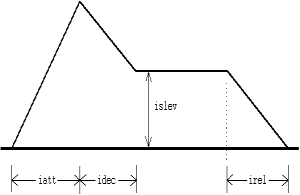
\includegraphics[scale=1]{adsr} 


 Picture of an ADSR envelope.


  The length of the sustain is calculated from the length of the note. This means \emph{adsr}
 is not suitable for use with MIDI events. The opcode \emph{madsr}
 uses the \emph{linsegr}
 mechanism, and so can be used in MIDI applications. The opcode \emph{mxadsr}
 is identical to \emph{madsr}
 except it uses exponential, rather than linear, line segments. 


 \emph{mxadsr}
 is new in Csound version 3.51. 
\subsection*{See Also}


 \emph{adsr}
, \emph{madsr}
, \emph{xadsr}

\subsection*{Credits}


 November 2002. Thanks to Rasmus Ekman, added documentation for the \emph{ireltim}
 parameter.


 November 2003. Thanks to Kanata Motohashi, fixed the link to the \emph{linsegr}
 opcode.
%\hline 


\begin{comment}
\begin{tabular}{lcr}
Previous &Home &Next \\
mute &Up &nchnls

\end{tabular}


\end{document}
\end{comment}
